\documentclass[conference]{IEEEtran}
\usepackage{graphicx}
\usepackage{booktabs}
\usepackage{amsmath}
\usepackage{listings}
\usepackage{xcolor}
\usepackage{url}
\usepackage{array}
\newcolumntype{L}[1]{>{\raggedright\arraybackslash}p{#1}}

\lstset{basicstyle=\ttfamily\footnotesize, columns=fullflexible, frame=single,
        breaklines=true, aboveskip=4pt, belowskip=4pt}
\newcommand{\TODO}[1]{\textbf{\textcolor{red}{TODO: #1}}}
\newcommand{\cell}[1]{\texttt{\detokenize{#1}}}

\begin{document}

\title{4-bit Unsigned Array Multiplier from RTL to GDSII\\
on SkyWater SKY130 with Open-Source Tools}

\author{\IEEEauthorblockN{Sai Poojith}
\IEEEauthorblockA{Roll No.\ 2025122010}
\and
\IEEEauthorblockN{Aneesh}
\IEEEauthorblockA{Roll No.\ 2025122002}}

\maketitle

\begin{abstract}
We designed a 4-bit $\times$ 4-bit unsigned array multiplier in Verilog
with registered inputs and outputs (16 flip-flops, 2-cycle latency),
verified it exhaustively, synthesised it to the SKY130
\cell{sky130_fd_sc_hd} library with Yosys, analysed its timing with
OpenSTA and took it to a GDSII layout with LibreLane. RTL and gate-level
simulation both pass all 256 input combinations. Synthesis gives 73 cells
(805.773\,$\mu$m$^2$) and STA gives $T_{\min}=2.596$\,ns
($F_{\max}=385.2$\,MHz) at the typical corner. LibreLane needed 8 runs
and closed timing at a 7.0\,ns clock across all its default corners, with
0 DRC and 0 LVS errors. Post-route $F_{\max}$ is 150.70\,MHz at the worst
(slow) corner and 302.91\,MHz at the typical corner.
\end{abstract}

% ======================================================================
\section{Part A --- RTL Design and Verification}

\subsection{Design}
\cell{rtl/full_adder.v} is a 1-bit full adder written only with
\texttt{assign} statements: $\mathit{sum}=a\oplus b\oplus c_{in}$ and
$c_{out}=ab+bc_{in}+ac_{in}$.
\cell{rtl/mult_array.v} registers \texttt{a} and \texttt{b} into
\cell{a_reg}/\cell{b_reg} (8 flip-flops), forms the 16 partial-product
bits $pp_i[j]=a[j]\wedge b[i]$, and adds them with three rows of four
\cell{full_adder} instances (\cell{fa_r1_0} \dots\ \cell{fa_r3_3}, 12 in
total) wired exactly as in the connection table of Section~2 of the
assignment. The 8-bit sum is registered into \texttt{p} (8 flip-flops).
All 16 flip-flops are cleared by the asynchronous active-low reset
\cell{rst_n}. No \texttt{*} operator is used in the design.
Fig.~\ref{fig:block} shows the block diagram.

\begin{figure*}[t]
\centering
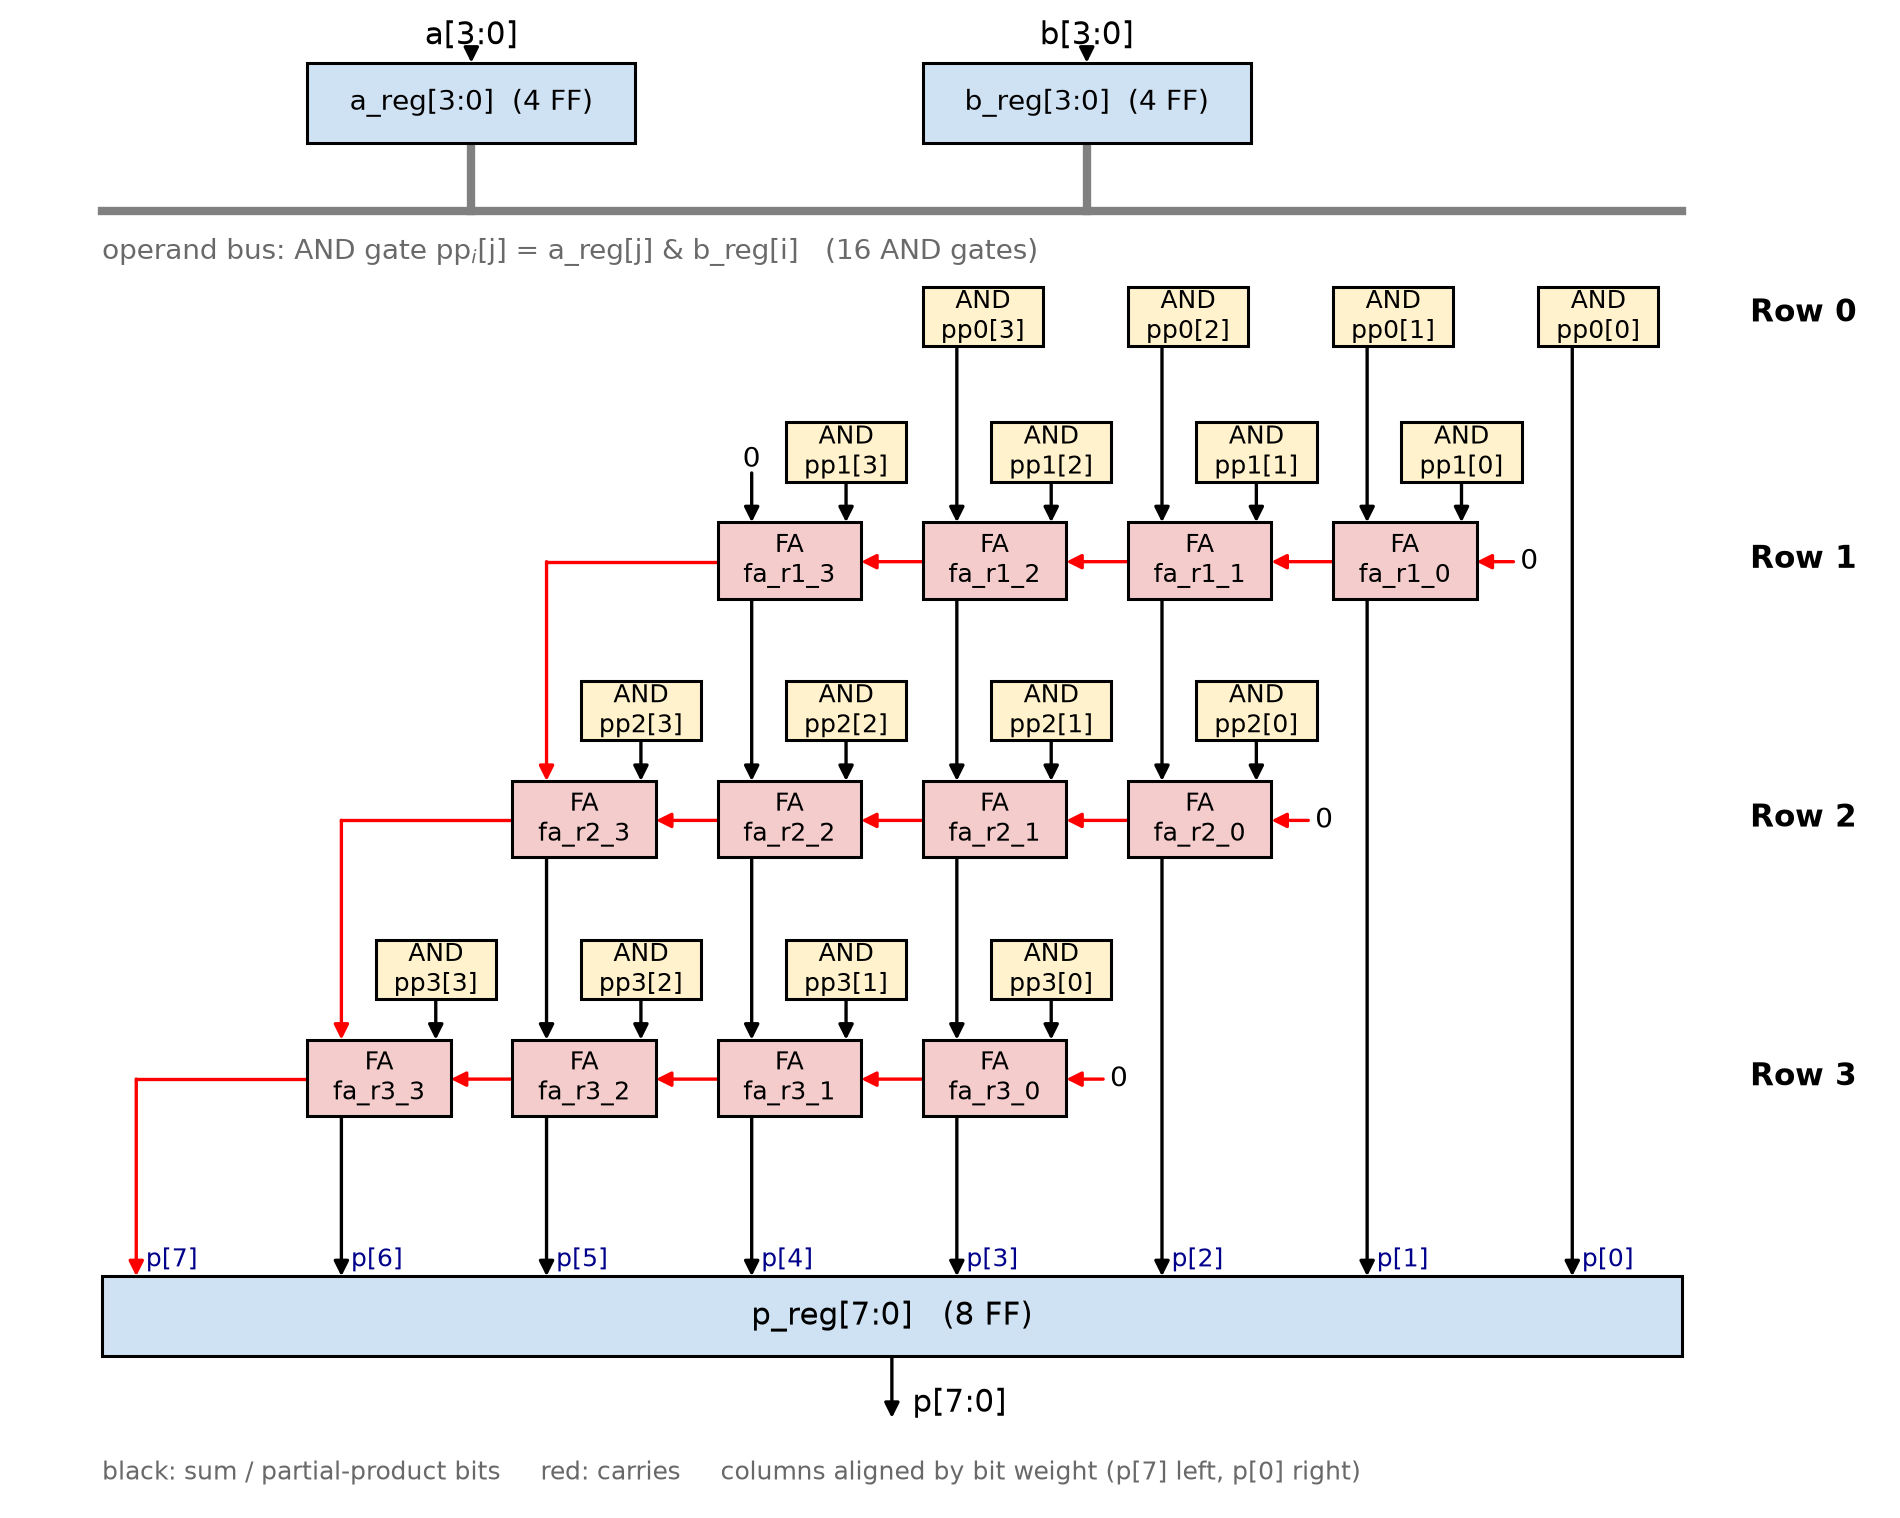
\includegraphics[width=0.82\textwidth]{figures/block_diagram.png}
\caption{Block diagram of \cell{mult_array}: input registers, the 16 AND
gates, the 12 full adders (labelled with their RTL instance names) and the
8-bit output register. Columns are aligned by bit weight; black arrows are
sum and partial-product bits, red arrows are carries.}
\label{fig:block}
\end{figure*}

\subsection{Testbench}
\cell{tb/tb_mult.v} generates a 10\,ns clock, holds \cell{rst_n} low for
the first two cycles and applies all 256 combinations of $a$ and $b$. Each
input is applied on a falling edge; the testbench waits two rising edges
(the 2-cycle latency) and compares \texttt{p} with \texttt{a*b} at the
next falling edge. It prints a line for every mismatch, one summary line
at the end, and dumps \cell{mult.vcd}.

\subsection{Results}
RTL simulation:
\begin{lstlisting}
PASS: 256 vectors checked, 0 errors
\end{lstlisting}
Error test (task 6), with \texttt{sum} changed to \verb|a ^ b|:
\begin{lstlisting}
MISMATCH: a=3 b=3 expected=9 got=5
...
FAIL: 256 vectors checked, 95 errors
\end{lstlisting}
After undoing the change the RTL simulation prints
\texttt{PASS: 256 vectors checked, 0 errors} again.

\subsection{Hand-worked example}
Sai Poojith's roll number 2025122010 ends in 0, so
$A = 0 + 5 = 5$ and $B = 7$.
\begin{lstlisting}[columns=fixed,keepspaces=true,breaklines=false]
        0 1 0 1  A = 5
      x 0 1 1 1  B = 7
---------------
        0 1 0 1  pp0 = A AND b0 (b0=1)
      0 1 0 1    pp1 = A AND b1 (b1=1), shifted 1
    0 1 0 1      pp2 = A AND b2 (b2=1), shifted 2
  0 0 0 0        pp3 = A AND b3 (b3=0), shifted 3
---------------
0 0 1 0 0 0 1 1  P = 35
\end{lstlisting}

Fig.~\ref{fig:wave} shows the same multiplication in GTKWave. The inputs
$a=5$, $b=7$ are applied at 1760\,ns, captured into the input registers at
clock edge~1 (1765\,ns), and the product $p=35$ appears after clock
edge~2 (1775\,ns): a latency of 2 clock cycles.

\begin{figure*}[t]
\centering
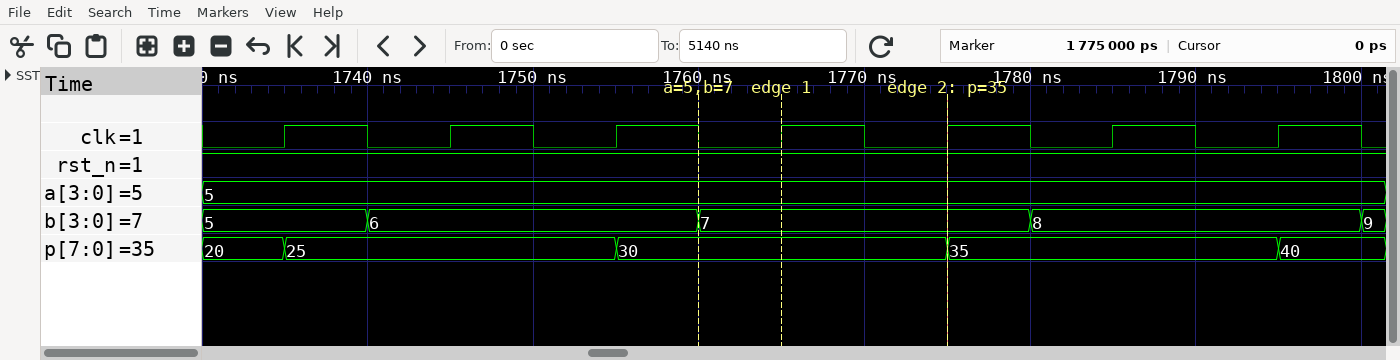
\includegraphics[width=\textwidth]{figures/waveform.png}
\caption{GTKWave view of the 5$\times$7 example (1730--1800\,ns). Marker
\emph{a=5,b=7}: inputs applied (1760\,ns); \emph{edge 1}: inputs captured
(1765\,ns); \emph{edge 2: p=35}: product registered (1775\,ns).}
\label{fig:wave}
\end{figure*}

% ======================================================================
\section{Part B --- Logic Synthesis}

\cell{synth/synth.tcl} runs the seven Yosys steps from the assignment
(\texttt{read\_verilog}, \texttt{synth -top mult\_array -flatten},
\texttt{dfflibmap}, \texttt{abc}, \texttt{opt\_clean -purge},
\texttt{stat}, \texttt{write\_verilog}) with the
\cell{tt_025C_1v80} Liberty file. Table~\ref{tab:synth} is taken from
\cell{synth/mult_array_stat.rpt}.

\begin{table}[h]
\caption{Part B results (Yosys)}
\label{tab:synth}
\centering
\begin{tabular}{@{}L{0.44\columnwidth}L{0.50\columnwidth}@{}}
\toprule
Metric & Value \\
\midrule
Total number of cells & 73 \\
Number of flip-flops & 16 (\cell{dfrtp_1}) \\
Total cell area ($\mu$m$^2$) & 805.773 \\
Flip-flop area ($\mu$m$^2$) & $16 \times 25.024 = 400.384$ \\
Flip-flop area (\% of total) & 49.69\,\% \\
3 most-used cell types & \cell{dfrtp_1} (16), \cell{nand2_1} (11), then a
four-way tie at 4: \cell{a21oi_1}, \cell{and2_0}, \cell{nand4_1},
\cell{xnor2_1} \\
Netlist simulation result & \texttt{PASS: 256 vectors checked, 0 errors} \\
\bottomrule
\end{tabular}
\end{table}

The gate-level netlist was simulated with the assignment's command
(\texttt{-DFUNCTIONAL -DUNIT\_DELAY=\#1}) and the same testbench, and
passed. Our first gate-level run printed
\texttt{FAIL: 256 vectors checked, 239 errors}. Every wrong value was the
product of the previous vector. The testbench was sampling \texttt{p}
1\,ns after the clock edge, which is exactly when the unit-delay
flip-flop models update their outputs. We moved the comparison to the
falling edge and reran all Part~A and Part~B simulations.

% ======================================================================
\section{Part C --- Static Timing Analysis}

\cell{sta/sta.tcl} runs the seven OpenSTA steps from the assignment at the
typical corner. At $T=10$\,ns the worst setup slack is 7.404\,ns, so
\begin{align*}
T_{\min} &= 10 - 7.404 = 2.596\ \text{ns},\\
F_{\max} &= 1000 / 2.596 = 385.2\ \text{MHz}.
\end{align*}
Rerunning with $T=2.60$\,ns gives a slack of 0.004\,ns (printed as
\texttt{worst slack max 0.00}), which confirms $T_{\min}$.

\begin{table}[h]
\caption{Part C results (OpenSTA, tt\_025C\_1v80)}
\label{tab:sta}
\centering
\begin{tabular}{@{}L{0.44\columnwidth}L{0.50\columnwidth}@{}}
\toprule
Metric & Value \\
\midrule
Worst slack at $T=10$\,ns (ns) & 7.404 \\
$T_{\min}$ (ns) & 2.596 (rerun at 2.60) \\
$F_{\max}$ (MHz) & 385.2 \\
Slack at $T=T_{\min}$ (ns) & 0.004 \\
Critical path start point & \cell{_118_} = \cell{b_reg[0]} (\cell{dfrtp_1}) \\
Critical path end point & \cell{_112_} = \cell{p_reg[6]} (\cell{dfrtp_1}, D = \cell{fa_r3_3.sum}) \\
Number of cells on the critical path & 10 (launch FF + 8 gates + capture FF) \\
Latency (ns) $= 2\times T_{\min}$ & 5.192 \\
Throughput (M results/s) & 385.2 \\
\bottomrule
\end{tabular}
\end{table}

\begin{table*}[t]
\caption{Cells on the critical path, in order (OpenSTA timing report, $T=2.60$\,ns)}
\label{tab:path}
\centering
\begin{tabular}{@{}rllrrl@{}}
\toprule
\# & Instance & Cell & Delay (ns) & Arrival (ns) & Role \\
\midrule
1 & \cell{_118_} & \cell{dfrtp_1} & 0.395 & 0.395 & launch flip-flop \cell{b_reg[0]} (CLK$\to$Q) \\
2 & \cell{_083_} & \cell{and2_0} & 0.212 & 0.607 & partial product $pp_0[0]=a[0]\wedge b[0]$ \\
3 & \cell{_055_} & \cell{or3_1} & 0.361 & 0.968 & adder carry logic \\
4 & \cell{_059_} & \cell{and4_1} & 0.215 & 1.183 & adder carry logic \\
5 & \cell{_070_} & \cell{o2111a_1} & 0.234 & 1.417 & adder carry logic (also takes $a[2]$, $b[2]$) \\
6 & \cell{_076_} & \cell{o21ai_0} & 0.216 & 1.634 & adder carry logic \\
7 & \cell{_090_} & \cell{xnor3_1} & 0.274 & 1.907 & 3-input XOR (full-adder sum) \\
8 & \cell{_091_} & \cell{maj3_1} & 0.375 & 2.282 & majority (full-adder carry) \\
9 & \cell{_092_} & \cell{xor3_1} & 0.178 & 2.460 & 3-input XOR = \cell{fa_r3_3.sum} \\
10 & \cell{_112_} & \cell{dfrtp_1} & setup 0.135 & --- & capture flip-flop \cell{p_reg[6]} \\
\bottomrule
\end{tabular}
\end{table*}

The path starts at \cell{b_reg[0]}, goes through the partial-product AND
gate for $pp_0[0]$, then through the carry logic of the adder rows, and
ends at the sum output of \cell{fa_r3_3}, which is \texttt{p[6]}.
In the netlist, \cell{_083_} really is $a[0]\wedge b[0]$ (it also drives
\cell{p_reg[0]}). In the RTL $pp_0[0]$ only drives $p[0]$, but row~1's
first carry $c_1[1]=pp_1[0]\,pp_0[1]=(a_0b_1)(a_1b_0)$ equals
$pp_0[0]\,pp_1[1]$, so ABC reused this AND gate in the carry logic (it
feeds \cell{_054_}--\cell{_057_} together with NAND$(a_1,b_1)$ and
NAND$(a_2,b_0)$).
Of the 8 logic gates, 1 is a partial-product AND gate and 7 (rows 3--9 in
Table~\ref{tab:path}) implement full-adder sum and carry logic. The
estimate in Section~2 is about $2N=8$ full-adder delays. Because the
design was flattened, ABC was free to merge adjacent full-adder stages
into larger single cells such as \cell{and4_1}, \cell{o2111a_1} and
\cell{xnor3_1}, so 7 cells cover the work of about 8 full-adder delays.

% ======================================================================
\section{Part D --- Physical Design}

\cell{pnr/config.json} contains exactly the six settings from the
assignment: \cell{DESIGN_NAME}, \cell{VERILOG_FILES}, \cell{CLOCK_PORT},
\cell{CLOCK_PERIOD}, \cell{FP_SIZING} = \texttt{"absolute"} and
\cell{DIE_AREA} = \texttt{[0, 0, 150, 150]}. The flow was run with
\texttt{librelane config.json} (LibreLane v3.1.0.dev3) and its default
timing corners: typical, slow and fast process corners
(\cell{tt_025C_1v80}, \cell{ss_100C_1v60}, \cell{ff_n40C_1v95}), each with
nominal, minimum and maximum wire parasitics.

\subsection{Timing closure}
The starting period was
$1.2\times T_{\min} = 1.2\times 2.596 = 3.115$\,ns, rounded up to
3.5\,ns. Every failing run failed only on setup timing in the slow corner
\cell{ss_100C_1v60}, where cells are much slower than at the typical
corner used in Part~C. Following the assignment, we increased
\cell{CLOCK_PERIOD} by 0.5\,ns after each failure (Table~\ref{tab:runs}).
From 3.5 to 5.5\,ns the slack improved by 0.5\,ns per run, but at 6.0
and 6.5\,ns it hardly improved. Synthesis was identical in all eight runs
(67 cells, 738.208\,$\mu$m$^2$), and so was the layout up to clock-tree
synthesis (1224.92\,$\mu$m$^2$ of standard cells). The runs differ only
in the post-CTS timing-repair step (\cell{ResizerTimingPostCTS}), which
upsizes gates only where it predicts a setup violation from pre-route
wire estimates. Up to 5.5\,ns it added 101.35\,$\mu$m$^2$ (to
1326.27\,$\mu$m$^2$); at 6.0\,ns it added only 73.83\,$\mu$m$^2$; at
6.5 and 7.0\,ns it predicted no violation and added nothing. With less
upsizing the slow-corner path got slower (data arrival 5.68\,ns up to
5.5\,ns, 6.13\,ns at 6.0\,ns, 6.66\,ns at 6.5\,ns), so the slack stayed
negative until 7.0\,ns, where the same un-upsized netlist met timing.

\begin{table}[h]
\caption{LibreLane runs (from each run's final metrics)}
\label{tab:runs}
\centering
\setlength{\tabcolsep}{4pt}
\begin{tabular}{@{}rrlrrr@{}}
\toprule
\# & Period & Result & Worst slack & Viol. & tt slack \\
   & (ns) &  & (ns), ss & & (ns) \\
\midrule
1 & 3.5 & FAIL & $-2.154$ & 15 & 0.587 \\
2 & 4.0 & FAIL & $-1.654$ & 12 & 1.087 \\
3 & 4.5 & FAIL & $-1.154$ & 12 & 1.587 \\
4 & 5.0 & FAIL & $-0.654$ & 9 & 2.087 \\
5 & 5.5 & FAIL & $-0.155$ & 3 & 2.587 \\
6 & 6.0 & FAIL & $-0.107$ & 3 & 2.899 \\
7 & 6.5 & FAIL & $-0.136$ & 3 & 3.199 \\
8 & 7.0 & PASS & $+0.364$ & 0 & 3.699 \\
\bottomrule
\end{tabular}\\[2pt]
{\footnotesize Worst corner in every run: \cell{max_ss_100C_1v60}.
tt = \cell{nom_tt_025C_1v80}. All runs: 0 DRC, 0 LVS.}
\end{table}

\subsection{Results}
Post-route $F_{\max} = 1000/(\text{CLOCK\_PERIOD} - \text{setup slack})$.
We give it both for the worst corner, which is what LibreLane signs off
on, and for the typical corner, which is the fair comparison with
Part~C:
\begin{align*}
\text{worst (ss): } & 1000/(7.0 - 0.3644) = 150.70\ \text{MHz},\\
\text{typical (tt): } & 1000/(7.0 - 3.6987) = 302.91\ \text{MHz}.
\end{align*}

\begin{table*}[t]
\caption{Part D results (LibreLane final run, 7.0\,ns clock)}
\label{tab:pnr}
\centering
\begin{tabular}{@{}L{0.30\textwidth}L{0.62\textwidth}@{}}
\toprule
Metric & Value \\
\midrule
CLOCK\_PERIOD used (ns) & 7.0 \\
Number of runs needed & 8 (3.5, 4.0, 4.5, 5.0, 5.5, 6.0, 6.5, 7.0\,ns) \\
Core area ($\mu$m$^2$) & 17\,759.5 (die area 22\,500) \\
Cells after synthesis (Part B) & 73 \\
Cells after place and route & 1895 (334 standard cells + 1561 fill/decap) \\
Kinds of cells added & decap 1314 (\cell{decap_12} 905, \cell{decap_6} 175, \cell{decap_3} 130,
\cell{decap_8} 55, \cell{decap_4} 49); fill 247 (\cell{fill_1} 215, \cell{fill_2} 32);
tap 245 (\cell{tapvpwrvgnd_1}); buffers 22: 17 I/O port buffers (\cell{buf_2}),
3 clock-tree buffers (\cell{clkbuf_16}), 2 fanout buffers (\cell{clkdlybuf4s50_1}) that split
the \cell{rst_n} net (16 reset pins, above the maximum fanout of 10) \\
Wirelength ($\mu$m) & 2362 \\
Setup slack (ns) & worst corner (\cell{max_ss_100C_1v60}): 0.3644;\quad typical (\cell{nom_tt_025C_1v80}): 3.6987 \\
Post-route $F_{\max}$ (MHz) & worst corner: 150.70;\quad typical corner: 302.91 \\
$F_{\max}$ from Part C (MHz) & 385.2 (typical corner, no wires) \\
DRC errors & 0 (Magic 0, KLayout 0) \\
LVS errors & 0 \\
\bottomrule
\end{tabular}
\end{table*}

The 1895 instances are 16 flip-flops and 51 logic cells from LibreLane's
own synthesis, plus 1828 cells added by the flow
(Table~\ref{tab:pnr}). LibreLane runs its own Yosys script, so its logic
(67 cells, 738.208\,$\mu$m$^2$) is not identical to our Part~B netlist
(73 cells). Hold timing
also passes in every corner (worst hold slack 0.141\,ns).
Figs.~\ref{fig:layfull} and~\ref{fig:layzoom} show the final layout.

\begin{figure*}[p]
\centering
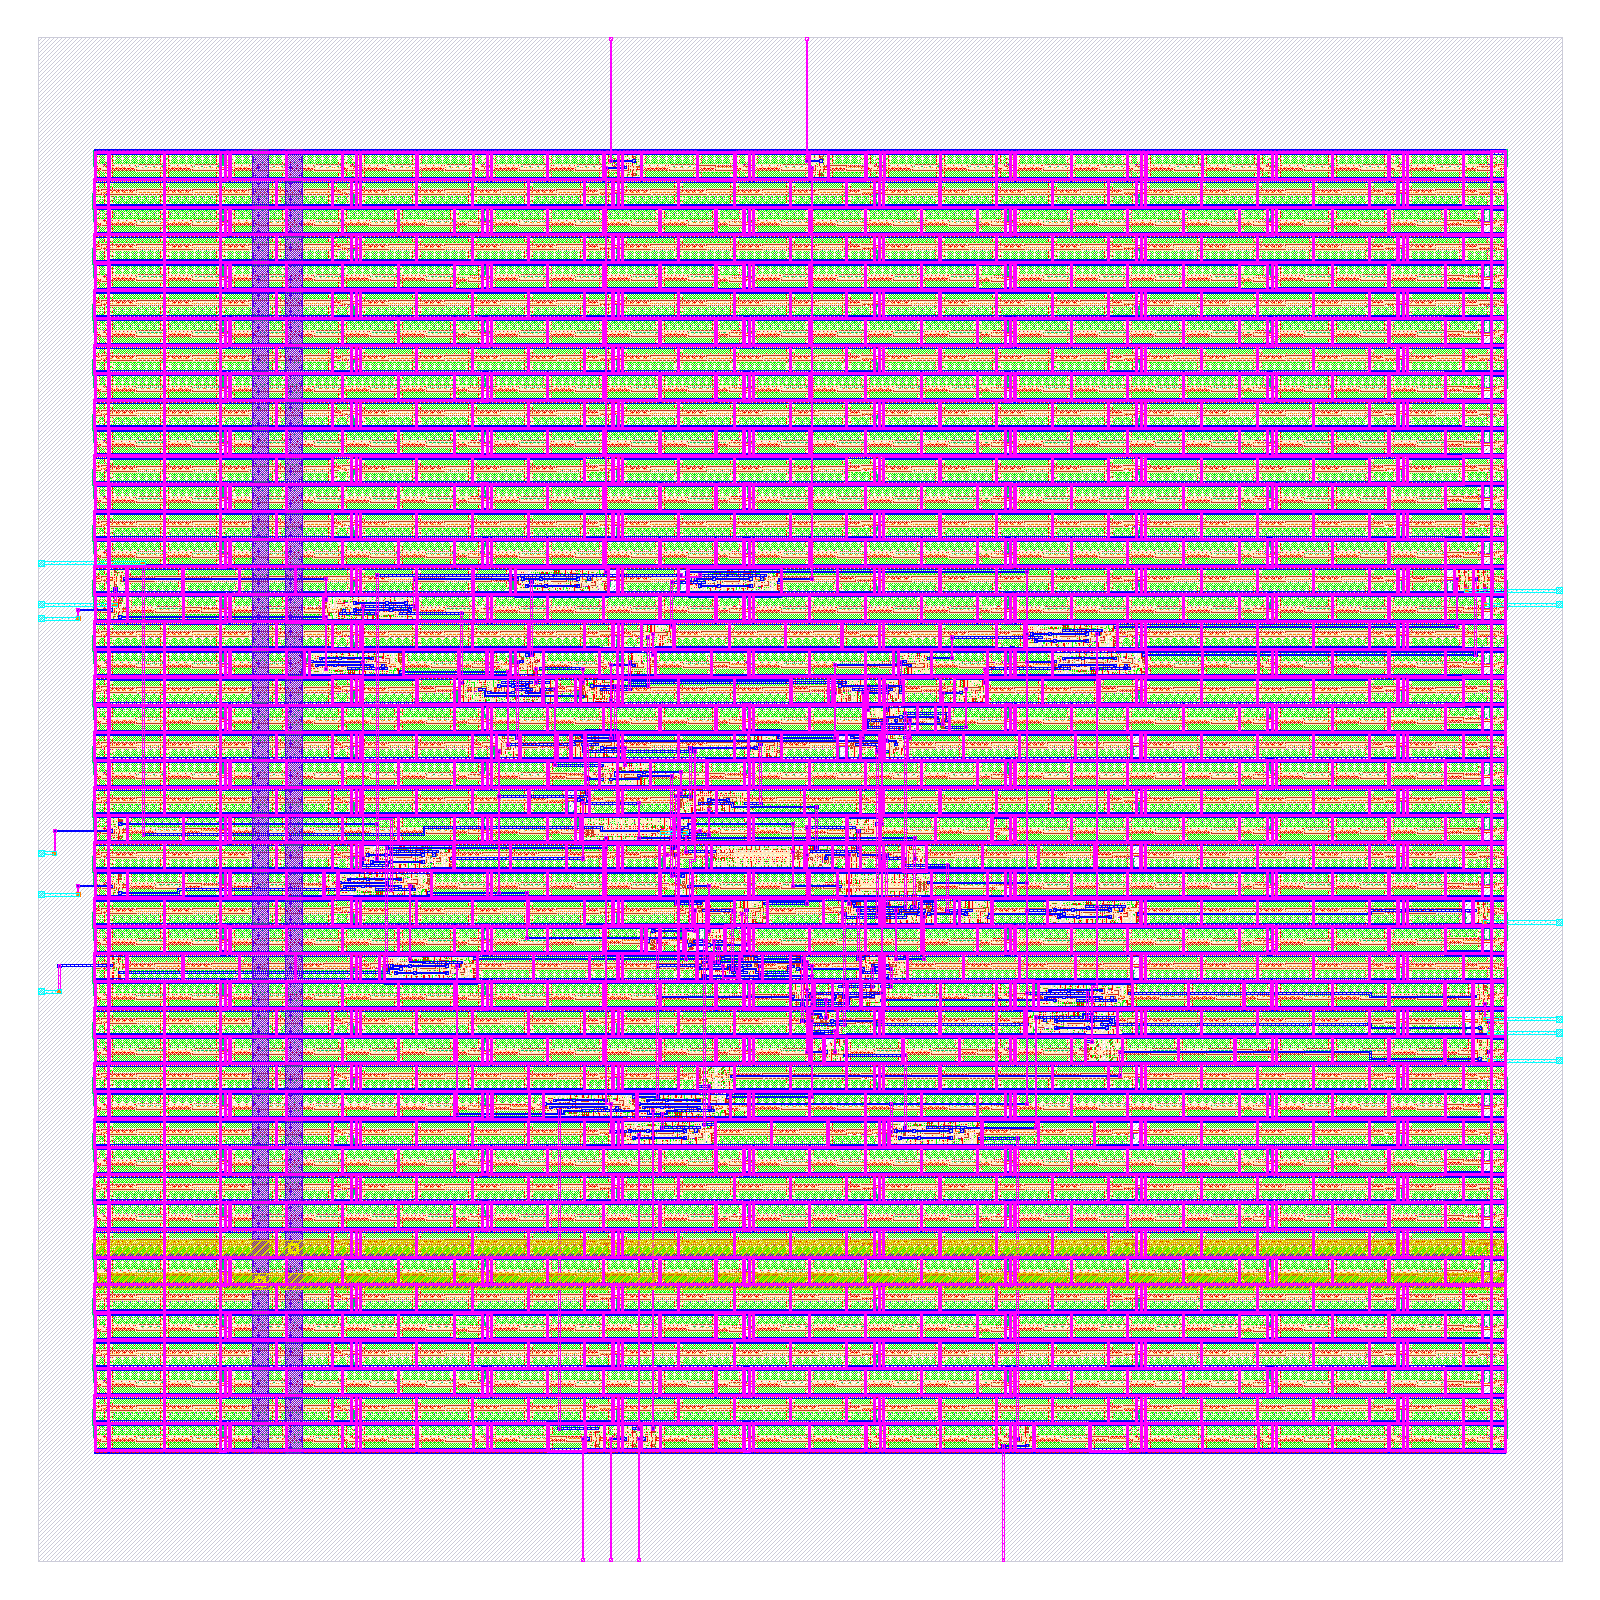
\includegraphics[width=0.56\textwidth]{figures/layout_full.png}
\caption{Whole 150$\times$150\,$\mu$m die (KLayout, \cell{pnr/mult_array.gds}).
The I/O pins sit on the die edge. The multiplier logic is clustered near
the centre, and the rest of the core rows are filled with decap, fill and
tap cells under the power grid.}
\label{fig:layfull}

\vspace{6pt}
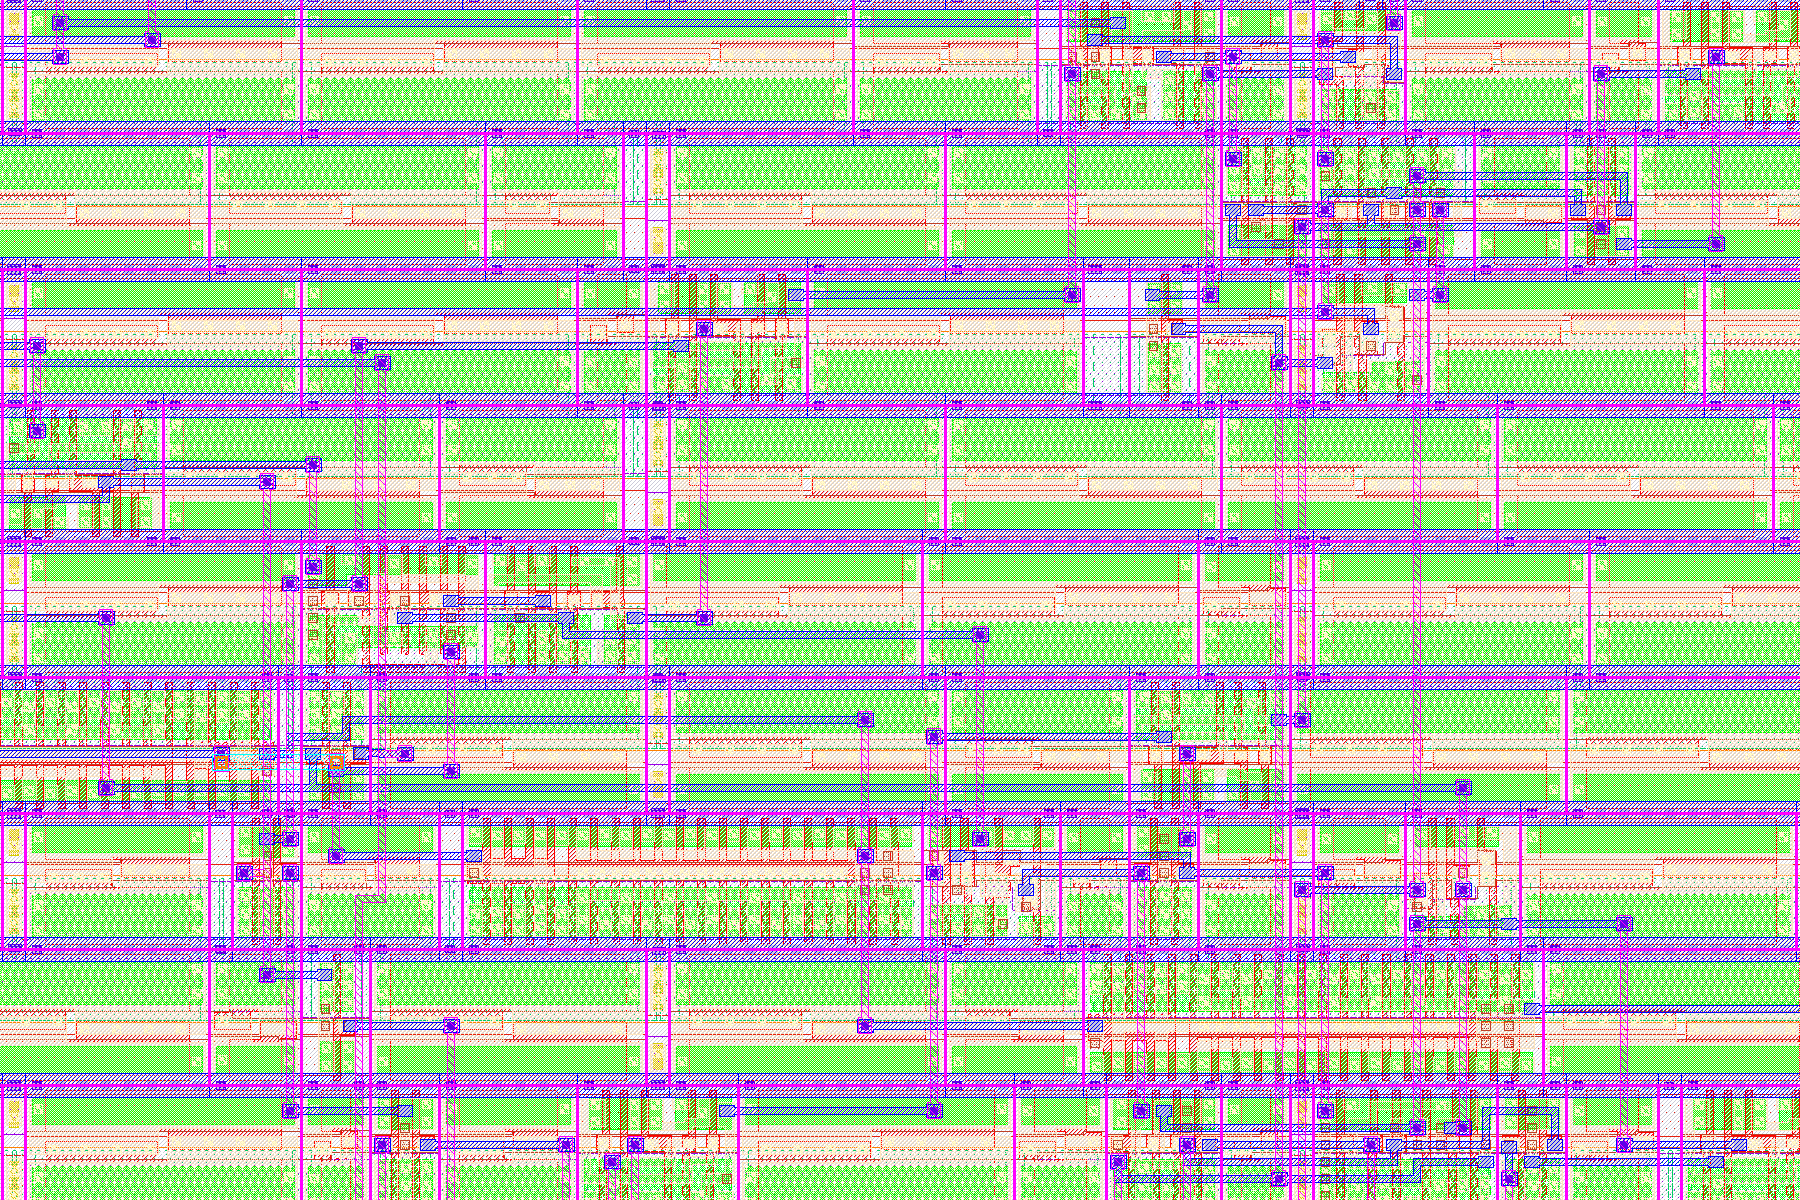
\includegraphics[width=0.86\textwidth]{figures/layout_zoom.png}
\caption{Zoomed 36$\times$24\,$\mu$m view at the die centre (colours from
\cell{sky130A.lyp}). Magenta outlines are the standard-cell boundaries
(areaid layer); the cells sit in horizontal rows with blue metal-1 power
rails along the row edges. Inside the cells, red is poly (transistor
gates), green is diffusion and pale beige is li1, the local-interconnect
layer that does most of the in-cell wiring (671\,$\mu$m$^2$ of li1 against
192\,$\mu$m$^2$ of metal-1 in this window). Blue metal-1, a few magenta
metal-2 wires and violet vias connect the cells.}
\label{fig:layzoom}
\end{figure*}

% ======================================================================
\section{Answers to Questions}

\textbf{Q1. Logic cells.}
Synthesis produced $73 - 16 = 57$ logic cells, about twice
$16 + 12 = 28$, because the RTL's AND gates and full adders do not map
one-to-one onto library cells. The design was flattened, so ABC optimised
all the logic together. It dropped constant inputs (each row's carry-in
and $r_0[3]$ are 0) and merged AND gates into adder logic
(\cell{o2111a_1} takes $a[2]$ and $b[2]$ directly). It also skipped the
library's multi-output \cell{fa_1} cell; its log says it ignored 9
multi-output cells. So each full adder becomes several single-output
cells, such as an XOR3 for the sum plus a MAJ3 or AND-OR cells for the
carry.

\textbf{Q2. Critical path.}
The critical path goes from input register \cell{b_reg[0]} (\cell{_118_})
to output register \cell{p_reg[6]} (\cell{_112_}, the sum of
\cell{fa_r3_3}). It has 10 cells: the launch flip-flop, 8 logic gates and
the capture flip-flop. The logic part takes $2.460 - 0.395 = 2.065$\,ns.
One gate is the partial-product AND for $pp_0[0]$, which ABC reused in
row~1's carry because $c_1[1]=pp_0[0]\,pp_1[1]$. The other 7
implement full-adder carry and sum logic, rippling through the rows to
\cell{fa_r3_3}. That is close to the $2N = 8$ full-adder estimate. It is
slightly fewer cells because ABC used complex gates (\cell{and4},
\cell{o2111a}, \cell{xnor3}, \cell{maj3}) that each do the work of more
than one simple full-adder stage.

\textbf{Q3. Flip-flop area.}
The flip-flops take 400.384 of 805.773\,$\mu$m$^2$, which is 49.69\,\%.
Each \cell{dfrtp_1} is 25.024\,$\mu$m$^2$, because it contains two latches
plus asynchronous reset logic. Most logic gates in our netlist are only
3.75--11.26\,$\mu$m$^2$; just the 3 \cell{xnor3}/\cell{xor3} cells are
close to a flip-flop in size (22.5--23.8\,$\mu$m$^2$). The design is tiny (57 logic cells), so the 16
registers are a large share. For an $N$-bit multiplier the logic grows
like $N^2$ but there are only $4N$ flip-flops, so in a bigger multiplier
this percentage would drop.

\textbf{Q4. Why post-route $F_{\max}$ is lower, and the added cells.}
Two effects lower it. The first is \emph{multi-corner signoff}. Part~C
used only the typical corner, but LibreLane signs off on its slowest
corner, \cell{ss_100C_1v60}. There, on the critical path from
\cell{a_reg[0]} (\cell{_102_}) to \cell{p_reg[6]} (\cell{_100_},
D~=~\cell{fa_r3_3.sum}), data arrives at 6.656\,ns instead of 3.247\,ns at
tt in the same layout, which gives the worst-corner $F_{\max}$ of
150.70\,MHz. The second is \emph{the real layout}: even at tt,
$F_{\max}$ falls from 385.2 to 302.91\,MHz. The tt effective period of
3.301\,ns is the 2.911\,ns data path (launch clock to D) plus a
0.124\,ns setup time, LibreLane's 0.25\,ns clock uncertainty and
0.016\,ns of clock skew. The capture clock arrives 0.034\,ns earlier
than the launch clock (0.302 vs.\ 0.336\,ns), less a 0.018\,ns
reconvergence credit. The clock-tree latency itself cancels, because it
delays both flip-flops. The data path is longer than Part~C's 2.460\,ns
for three reasons. Routed wires add RC, so the launch flip-flop's
clk$\to$Q is 0.472\,ns instead of 0.395\,ns. LibreLane's own synthesis
gives a different 9-gate path. And at 7.0\,ns the post-CTS timing repair
saw no violations, so it upsized nothing. The flow also added cells: 245
tap cells tie the n-wells and substrate to VPWR/VGND to prevent latch-up,
and 1314 decap cells are on-chip capacitors that steady the supply when
many gates switch. 247 fill cells close the gaps in the rows so wells,
implants and power rails stay continuous, and 3 \cell{clkbuf_16} cells
form the clock tree that reaches all 16 flip-flops with low skew. Finally,
there are 17 \cell{buf_2} buffers on the input and output ports and 2
fanout buffers that split \cell{rst_n}, whose 16 reset pins exceed the
maximum fanout of 10.

\textbf{Q5. DRC and LVS.}
DRC (design rule check) verifies that the layout geometry obeys the
foundry's manufacturing rules: minimum widths and spacings of each layer,
enclosures, via sizes, densities and so on. LVS (layout versus
schematic) extracts the transistors and connections from the layout and
checks that they match the netlist, so the layout is the circuit we
designed. Both must pass because they catch different failures. A
DRC-clean layout can still be the wrong circuit, and a layout that
matches the schematic can still be impossible to manufacture reliably
(shorts, opens, low yield). Our final layout has 0 DRC errors (Magic and
KLayout) and 0 LVS errors.

\textbf{Q6. Scaling to 8 bits.}
From Section~2, an $N$-bit array multiplier uses $N^2$ AND gates and
$N(N-1)$ full adders, and its longest path is about $2N$ full-adder
delays.
\begin{align*}
N=4:&\quad 4\cdot3 = 12\ \text{FAs},\quad 2\cdot4 = 8\ \text{FA delays}\\
N=8:&\quad 8\cdot7 = 56\ \text{FAs},\quad 2\cdot8 = 16\ \text{FA delays}
\end{align*}
So the number of full adders grows by $56/12 \approx 4.7\times$ (and the
AND gates from 16 to 64), but the critical path only doubles. Scaling
our Part~C logic delay: $T_{\min} \approx 0.395 + 2\times 2.065 + 0.135
\approx 4.66$\,ns, so $F_{\max}$ would drop from about 385\,MHz to about
215\,MHz at the typical corner. Here 0.395\,ns is the clk$\to$Q delay,
2.065\,ns is the logic delay and 0.135\,ns is the setup time. The area
grows roughly quadratically and the delay roughly linearly.

\end{document}
